% !TEX TS-program = pdflatex
% !TEX encoding = UTF-8 Unicode

% This is a simple template for a LaTeX document using the "article" class.
% See "book", "report", "letter" for other types of document.

\documentclass[11pt]{llncs} % use larger type; default would be 10pt

\usepackage[utf8]{inputenc} % set input encoding (not needed with XeLaTeX)

%%% Examples of Article customizations
% These packages are optional, depending whether you want the features they provide.
% See the LaTeX Companion or other references for full information.

%%% PAGE DIMENSIONS
\usepackage{geometry} % to change the page dimensions
\geometry{a4paper} % or letterpaper (US) or a5paper or....
% \geometry{margin=2in} % for example, change the margins to 2 inches all round
% \geometry{landscape} % set up the page for landscape
%   read geometry.pdf for detailed page layout information

\usepackage{graphicx} % support the \includegraphics command and options

% \usepackage[parfill]{parskip} % Activate to begin paragraphs with an empty line rather than an indent

\usepackage{mathtools}
\usepackage{mathpartir}
\usepackage{times}
\usepackage{amssymb}
\usepackage{float}
%%% PACKAGES
\usepackage{booktabs} % for much better looking tables
\usepackage{array} % for better arrays (eg matrices) in maths
\usepackage{paralist} % very flexible & customisable lists (eg. enumerate/itemize, etc.)
\usepackage{verbatim} % adds environment for commenting out blocks of text & for better verbatim
\usepackage{subfig} % make it possible to include more than one captioned figure/table in a single float
% These packages are all incorporated in the memoir class to one degree or another...

\usepackage{cite}

%%% HEADERS & FOOTERS
\usepackage{fancyhdr} % This should be set AFTER setting up the page geometry
\pagestyle{fancy} % options: empty , plain , fancy
\renewcommand{\headrulewidth}{0pt} % customise the layout...
\lhead{}\chead{}\rhead{}
\lfoot{}\cfoot{\thepage}\rfoot{}

%%% SECTION TITLE APPEARANCE
\usepackage{sectsty}
\allsectionsfont{\sffamily\mdseries\upshape} % (See the fntguide.pdf for font help)
% (This matches ConTeXt defaults)

%%% ToC (table of contents) APPEARANCE
\usepackage[nottoc,notlof,notlot]{tocbibind} % Put the bibliography in the ToC
\usepackage[titles,subfigure]{tocloft} % Alter the style of the Table of Contents
\renewcommand{\cftsecfont}{\rmfamily\mdseries\upshape}
\renewcommand{\cftsecpagefont}{\rmfamily\mdseries\upshape} % No bold!

%%% END Article customizations

%%% The "real" document content comes below...

\title{An embedding of Concrete Data Structures into Dialogue Games}
\author{Clément Jacq and Paul-André Melliès\\}
\date{} % Activate to display a given date or no date (if empty),
         % otherwise the current date is printed 
\institute{Laboratoire IRIF, Université Paris Diderot}





\begin{document}
\maketitle
\section*{Abstract}
Dialogue games were recently introduced by Mellies [2014-2016]
as an attempt to unify the two traditional (but still disconnected)
frameworks for game semantics:
\begin{itemize}

\item concrete data structures and sequential algorithms introduced by Berry and Curien in the early 1980s
\item arena games introduced by Hyland, Nickau and Ong in the mid 1990s.
\end{itemize}

The key idea underlying the notion of dialogue game is that every move~$m$ 
of an arena game should be decomposed as a pair $m=(alpha,val)$
consisting of a cell $\alpha$ and of a value~$val$.\\
This decomposition enables one to interpret every move $m$ of an arena game 
as the action for Player or for Opponent of filling a given cell with a given value.
An important novelty of dialogue games with respect to concrete data structures
is that a cell or a value may be either Opponent or Player.
The only constraint is that a value should always fill a cell of the same polarity,
and that it should always justify a cell of the opposite polarity.\\

Once understood this decomposition of an arena move as a pair consisting
of a cell and of a value, the connection between dialogue games and arena games becomes essentially immediate. Despite the fact that they share the same philosophy of cells and values,
the connection between dialogue games and concrete data structures is more subtle. \\

In this talk, we will explain how to connect the sequential algorithm model designed
by Berry and Curien in the early 1980s with this recent notion of dialogue games.
To that purpose, we start from the nice graph game model of intuitionistic linear logic
designed by Hyland and Schalk in the early 2000s.\\  
We exhibit a number of interesting and sometimes unexpected structures of this model
by embedding it into a specific intuitionistic hierarchy of dialogue game.
This embedding enables us to recover the graphical notations of positions in dialogue games.
Take for instance the game $A=(Bool \otimes Bool) \multimap Bool$.
The translation as a graph:
\begin{figure}[H]\centering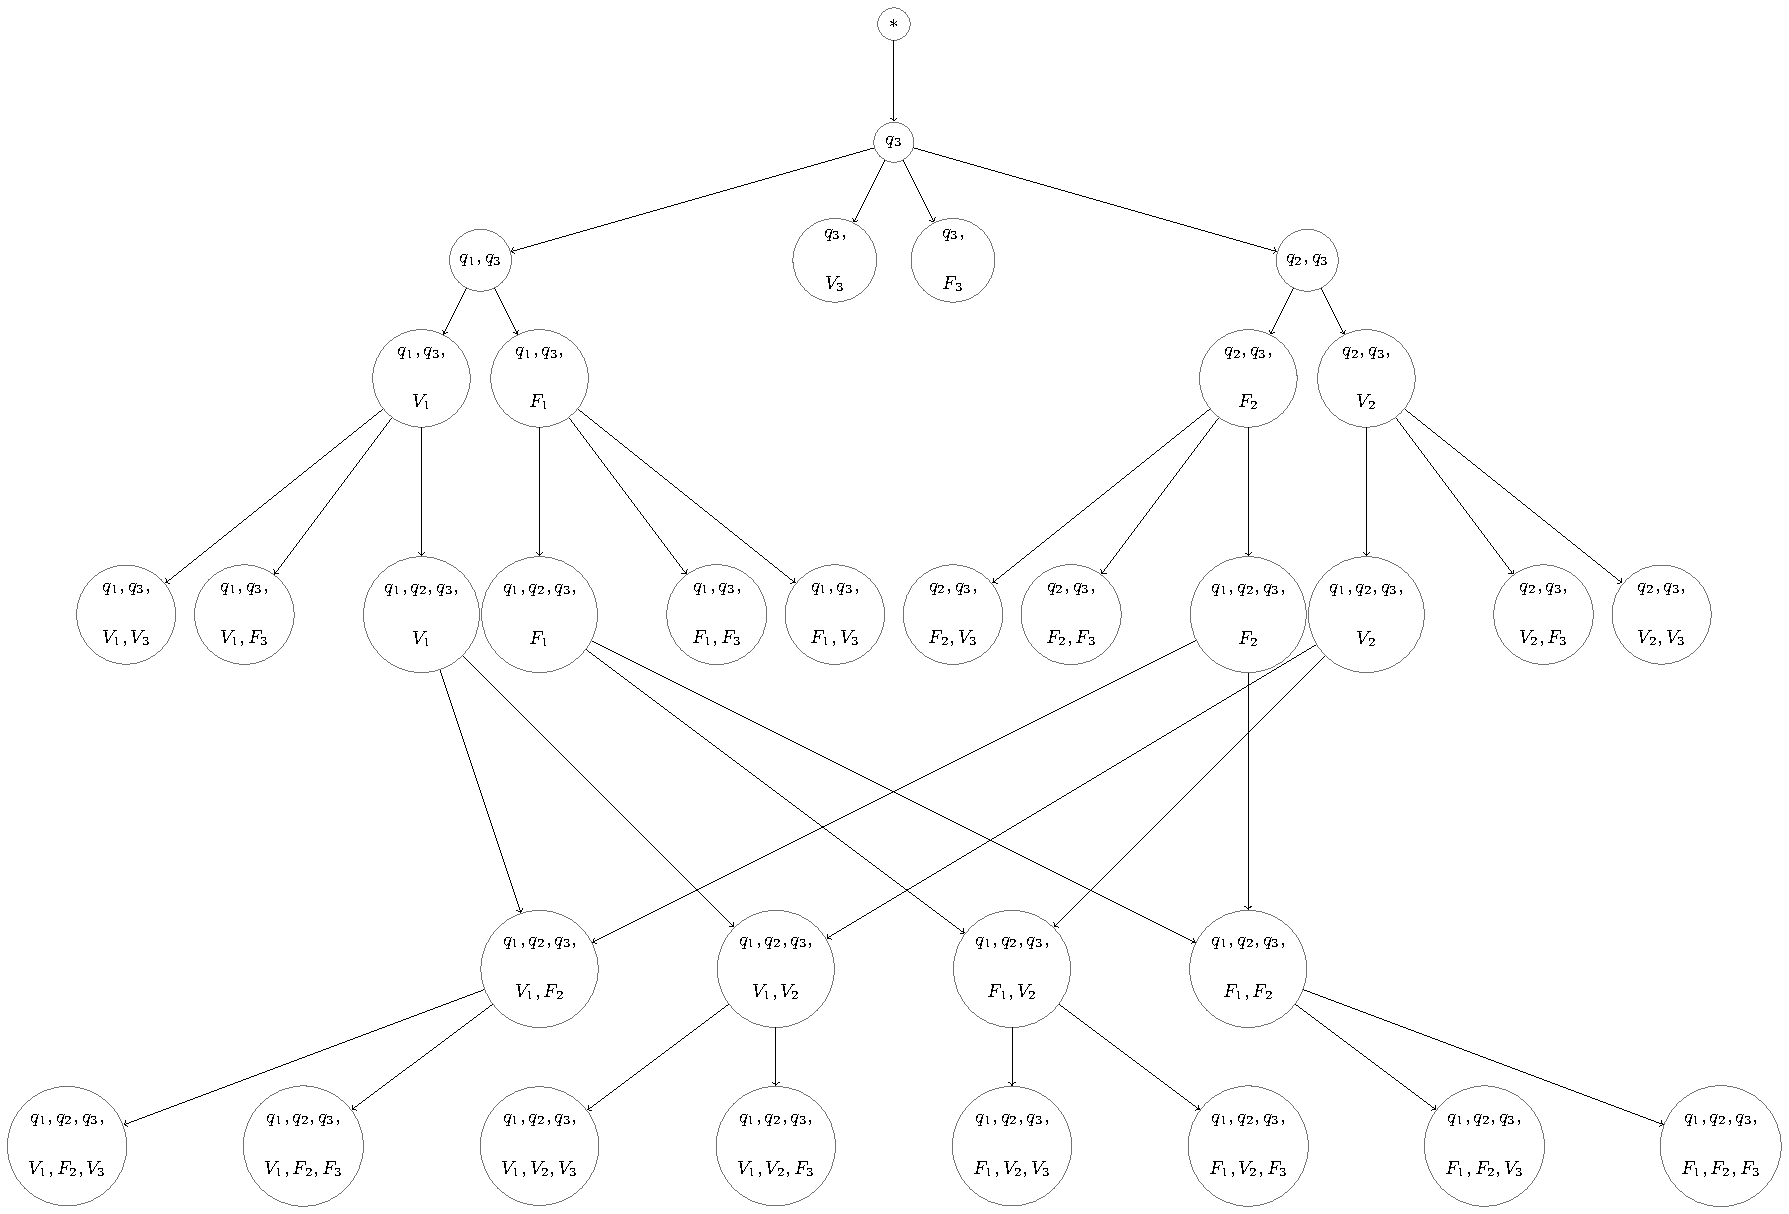
\includegraphics[scale=0.46]{bool-tens-bool-arrow-bool-graph.pdf}\caption{The graph game for the type $(Bool \otimes Bool) \multimap Bool$} \end{figure}


By embedding it in the dialogue game $B = \neg ( (\neg \neg (1+1)) \otimes (\neg \neg (1+1)) \otimes \neg (1+1))$
every position $x$ of the graph game $A$ may be depicted as follows:
\begin{figure}[H]\centering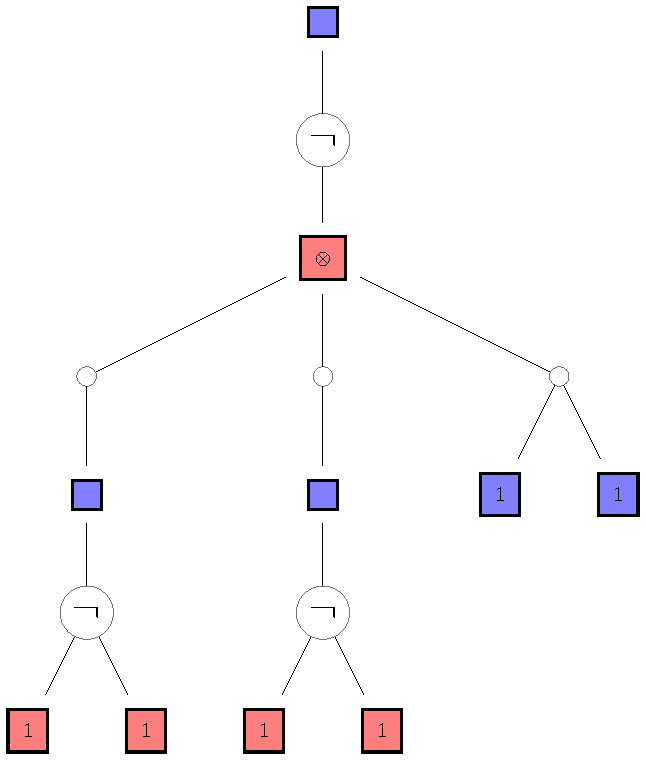
\includegraphics[scale=0.45]{bool-tens-bool-arrow-bool-dialogue.pdf}\caption{The dialogue game for the type $(Bool \otimes Bool) \multimap Bool$} \end{figure}

  

\bibliography{biblio}
\bibliographystyle{plain}
\end{document}
